\documentclass[prd, nofootinbib, floatfix, 12pt,tightenlines]{revtex4}
%\documentclass[useAMS,usenatbib,tightenlines,11pt,preprint]{aastex}
%testing push


\usepackage[paperwidth=8.5in,paperheight=11in,centering,hmargin=1in,vmargin=1in]{geometry}
\usepackage{amsmath}
\usepackage{amsbsy}

\topmargin0.0cm
\textheight8.5in


\input epsf
\usepackage{amsmath,amssymb,subfigure}
\usepackage{graphicx}
\usepackage{epsfig}
\usepackage{color}
%\usepackage{ulem}
%\usepackage{epstopdf}

\renewcommand{\topfraction}{0.95}
\renewcommand{\bottomfraction}{0.95}





%%%%%%%%%%%%%%%%%%%%%%%%%%%%%%%%%%%%%%%%%%%%%%%%%%%%%%%%%%%%
%%%%%%%%%%%%%%%%%%%%%%%%%%%%%%%%%%%%%%%%%%%%%%%%%%%%%%%%%%%%
%%%%%%%%%%%%%%%%%%%%%%%%%%%%%%%%%%%%%%%%%%%%%%%%%%%%%%%%%%%%

\begin{document} 
\sloppy
\title
{An Active Learning Approach to Optimizing Astronomy
}

%\pagerange{\pageref{firstpage}--\pageref{lastpage}}

\label{firstpage}

% \date{\today}

\maketitle 

%%%%%%%%%%%%%%%%%%%%%%%%%%%%%%%%%%%%%%%%%%%%%%%%%%%%%%%%%%%%
%%%%%%%%%%%%%%%%%%%%%%%%%%%%%%%%%%%%%%%%%%%%%%%%%%%%%%%%%%%%
%\begin{abstract} 

%\end{abstract} 

\section{Introduction}

{\bf Need a discussion of all the different sciences that will need some
kind of automated classification in the future}

\section{Photometric Redshifts}
\label{sec:photoz}

The apparent acceleration of the rate of cosmic expansion {\bf [CITE]}
represents one of the most vexing problems in modern astrophysics.
Whether it is an indication of the presence of a gravitationally-repulsive
``Dark Energy'' or of a break down in our General Relativistic description of
gravity, answering it will require a detailed three-dimensional map of the
constituents of the Universe, and how they are being moved away from us by the
cosmic expansion.  Traditionally, such measurements are made by taking detailed
spectra of objects and measuring the Doppler shift due to cosmic expansion (the
``redshift'' of the object, since cosmic expansion increases the wavelength of
emitted photons).
Detailed spectroscopy is an expensive measurement.  Photometry -- measuring the
brightness of objects in broad passband filters -- is thousands of times less
expensive.  Therefore, a great deal of attention has focused on developing a
method of determining ``photometric redshifts'': inferring a relationship
between an object's photometric and spectroscopic signatures such that redshifts
can be determined solely from photometric data.  

Presently, photometric redshifts are principally determined using
forward-fitting models.  Astronomers assume that they can model the rest frame
spectra of any galaxy.  These spectral models are
redshifted and integrated over the profile of an experiment's
photometric filters until a good fit to the observed photometric data is
found.  The redshift of the galaxy is taken as that which produces the best fit
between template and data.  Many publicly available codes such as 
EAZY \cite{eazy} implement this method.  
While it is straightforward in principle, it requires
accurate foreknowledge to select the appropriate basis spectra.  If the chosen
spectra are not representative of the population of observed
galaxies, the algorithm will fail to give accurate redshifts and cosmological
inferences will be inaccurate \cite{budavari2008}.  The effects of this
shortcoming can be seen in Figure \ref{subfig:eazy}, which plots the results
of running the publically available EAZY algorithm \cite{eazy} on a set of
simulated galaxy observations designed to represent results expected from the
Large Synoptic Survey Telescope (LSST\footnote{http://www.lsst.org}).
While many of the galaxies fall near the
$z_\text{photometric}=z_\text{spectroscopic}$ line, there is significant scatter
in the results.  We propose to overcome this difficulty with an exclusively
data-driven algorithm based on Gaussian Processes.


\begin{figure}
\subfigure[]{
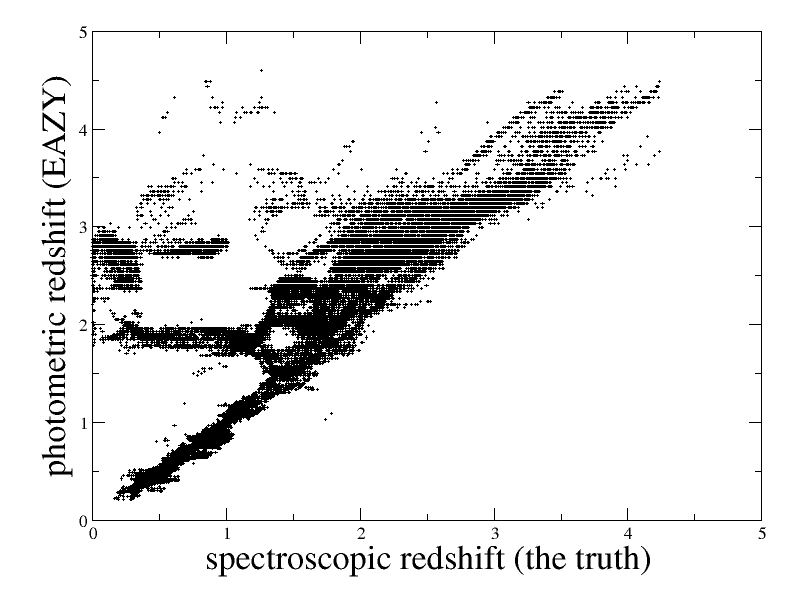
\includegraphics[scale=0.2]{eazy_scatter_plot.png}
\label{subfig:eazy}
}
\subfigure[]{
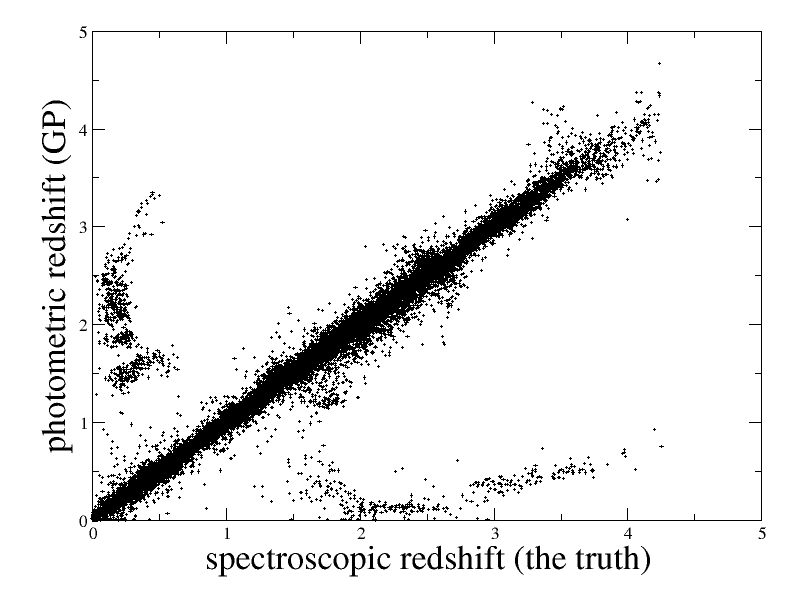
\includegraphics[scale=0.2]{gp_scatter_plot.png}
\label{subfig:gp}
}
\caption{
Photometric redshift plotted
against true spectroscopic redshift for 48,000 simulated LSST galaxy
observations.  Photometric redshifts are derived using the
EAZY template-fitting
algorithm in Figure \ref{subfig:eazy} and
our Gaussian Process based algorithm in Figure \ref{subfig:gp}.
}
\label{fig:scatter}
\end{figure}

We treat the photometric redshift problem probabilistically.  Rather than
taking the spectroscopic data and learning a one-to-one photometric redshift
relationship, we will use Gaussian Processes to model a probability density
function in $P(z_\text{photometric})$ which can characterize the probability that a
given galaxy is at a given redshift.  This method will not only be resilient
against the pitfalls demonstrated in Figure \ref{subfig:eazy}, but will allow us
to quantify the information content of our trainind data in such a way as to
optimize the gathering of additional spectroscopic data to further improve on
our results.  
Figure \ref{subfig:gp} shows preliminary results from our
algorithm when trained on spectroscopic data from an 
additional 50,000 galaxies.
We discuss specifically how we model $P(z_\text{photometric})$ below.

\subsection{Gaussian Processes}
\label{sec:gppz}

Gaussian processes (GPs) are means for interpolating the value of a scalar
function on high-dimensional coordinate spaces given noisy data \cite{gp}.
An important feature of GPs is that they do not make parametric assumptions
about the form of the function they are modeling.  They have received
attention as a means of describing physical phenomena (e.g. the expansion
history of the universe) without having to assume a model of the underlying
process \cite{ericgp}, of interpolating point spread functions across large
images \cite{psf}, and of accelerating the search of high-dimensional
likelihood functions on the cosmological parameters by efficiently
selecting sample points \cite{daniel2012}.  We illustrate the method below for the
case of photometric redshifts.

Assume that each galaxy training set datum is of the form
$\{\vec{\theta},y\}$, where $\vec{\theta}$ is an $N_p$-dimensional vector
respresenting the magnitude of the galaxy in each of the survey's filters
(the galaxy's position in photometric color space) and $y = f(\theta)$ is
the physical quantity (redshift) we are trying to infer.  Gaussian
processes assume that $f$ is a probabilistic function on the
$N_p$-dimensional space with some covariance function such as a squared
exponential covariance,
$K_{ij}\equiv\text{Cov}\left[f(\vec{\theta}^{i}),f(\vec{\theta}^{j})\right]
= \exp(-\frac{1}{2}|\vec{\theta}^{i} - \vec{\theta}^{j}|^2)$.
Under those assumptions, the mean of the predicted redshift distribution
for a new query point $\{\vec{\theta}^{q}\}$ is:

\begin{equation}
f(\vec{\theta}^{q}) = \sum_{i=1}^n \
\alpha_i k(\vec{\theta}^{i},\vec{\theta}^{qi})
\label{eq:mean}
\end{equation}

\noindent
where $\vec{\alpha} = (K + \sigma^2 I)^{-1}\vec{y}$, $K$ is the matrix of
covariances between all training points, $\sigma^2$ is the variance of
Gaussian noise added to each observed value of $y$, and $\vec{y}$
represents the training data redshifts.  The variance of the predicted
redshift distribution is:

\begin{equation}
\Sigma^{q} = \text{Cov}(f^{q}) = K_{qq} - K_q^T (K + \sigma^2I)^{-1} K_q
\label{eq:cov}
\end{equation}

\noindent
where $K_q$ is the vector of covariances between the query point and all
training points.  Eq. \ref{eq:cov} extends directly to the case of multiple
query points by making the variables matrices as appropriate, and the
result is a full covariance matrix for the query points.  Readers looking
for a more detailed explanation of Gaussian processes should consult
Rasmussen and Williams (2006).

Gaussian processes offer two distinct advantages which render them particularly
amenable to integration into active learning frameworks.
Because they model the likelihood of both their inputs and their outputs, they
allow us to assess both our confidence in the outputs (the probability that we
have found the correct photometric redshift), and our confidence in the model as
a whole.
Bryan {\it et al}. (2007) and Daniel {\it et al}. (2012) use the former 
feature to great affect, treating the determined variances as a
measure of the information that can be learned by promoting a query point
to a new training point and thus learning the likelihood surface of a
theory space with greater efficiency than traditional MCMC methods (see
especially Figures 5-10 of Daniel {\it et al}. 2012).
The latter feature allows us to compare PDF models with one and two modes, thus
correcting for the degeneracies in the photometry-to-redshift relationship in
Figure \ref{subfig:annz}.  This is the method we use to generate Figure
\ref{fig:gp}.

The second advantage of Gaussian processes is their indifference to the
physical meaning of the inputs and outputs.  There is nothing to prevent us
from adding other variables into $\vec{\theta}^{i}$ and including them
into the covariance structure of $K_{ij}$. As presented, $K_{ij}$ was the
redshift-redshift correlation function.  We could just as easily include
redshift-magnitude and magnitude-magnitude correlation functions.  
Indeed, Gaussian processes allow us to incorporate any measured attribute (e.g.
morphology, nearest-neighbor distance) of our galaxies in a principled manner
and use those attributes to control the spread and bias in our redshift
determination.
In this
way, we can incorporate the measurement uncertainties in our photometric
colors and propagate them consistently through to uncertainties in the
determined photometric redshifts.  This would directly address the
shortcomings of present Gaussian Process methods identified by Bonfield
{\it et al}. (2010) vis-\`a-vis error propagation.

\begin{figure}
\subfigure[]{
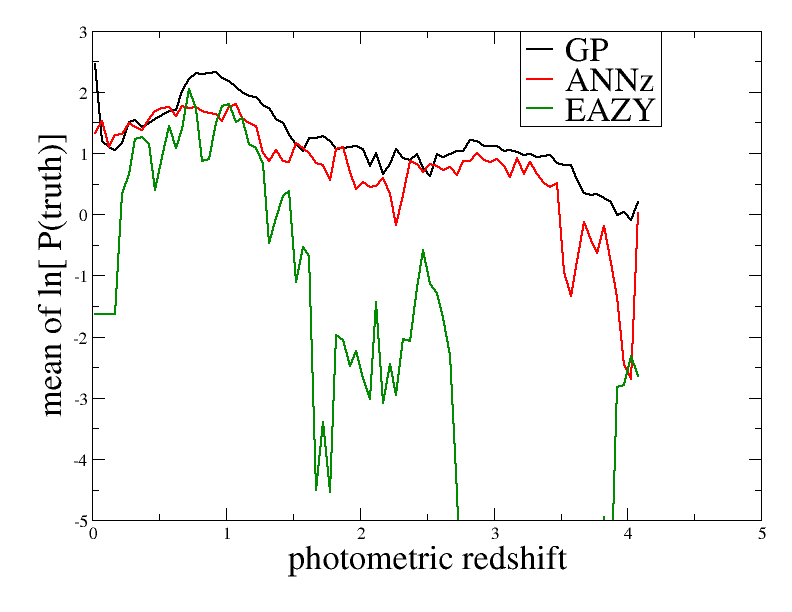
\includegraphics[scale=0.2]{lnsum_lsst.png}
\label{subfig:lnsumlsst}
}
\subfigure[]{
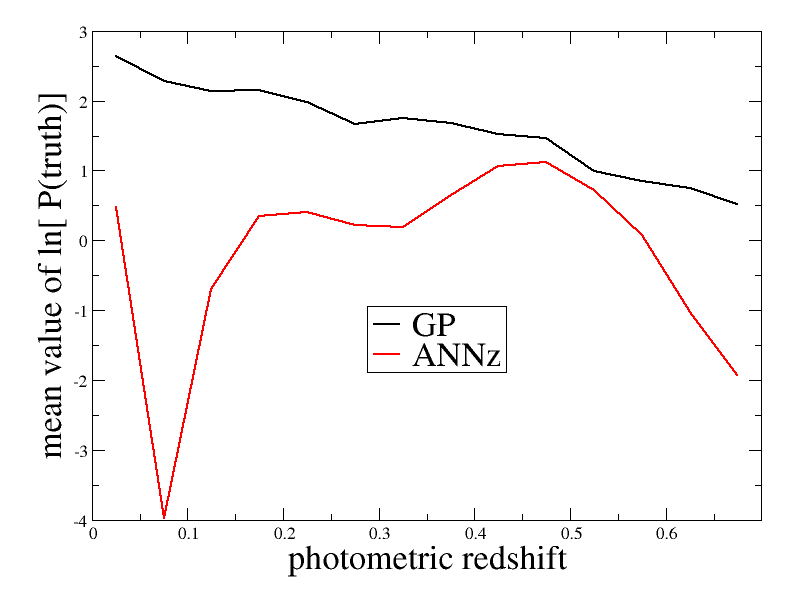
\includegraphics[scale=0.2]{sdss_lnsum.png}
\label{subfig:lnsumsdss}
}
\caption{
Figure \ref{subfig:lnsumlsst} shows the mean value of
$\ln[P(\text{truth})]$ as a function of photometric redshift (the vertical
axes in Figures \ref{fig:scatter}) for all
three algorithms under consideration.  
Figure \ref{subfig:lnsumsdss} compares our Gaussian Process method
to the artificial neural network code ANNz \cite{annz} on real
data taken from the Sloan Digital Sky Survey.  In this latter case, the
algorithms are trained on 70,000 galaxies and tested on 715,000 galaxies.
}
\label{fig:gp}
\end{figure}

Figure \ref{fig:gp} shows preliminary results of our proposed probabilistic
Gaussian Process algorithm.  Figure \ref{subfig:gpscatter} plots photometric
redshift versus spectroscopic redshift for the same simulated
galaxy observations used in Figure
\ref{fig:scatter}.  
According to this metric,
Gaussian Processes perform better than the EAZY algorithm
and comparably to the neural network of ANNz.  However, if we instead measure
performancy by considering $\ln[P(\text{truth})]$, i.e. the logarithm of the
value of the posterior probability density function at the known spectroscopic
redshift of our galaxies, we see that Gaussian Processes consistently outperform
neural networks (see Figure \ref{subfig:lnsumlsst}).
Figure \ref{fig:sdss} recreates Figure \ref{subfig:lnsumlsst} using actual data
taken from the Sloan Digital Sky Survey \cite{Abazajian:2008wr}.

Other data-driven algorithms for photometric redshift determination do exist. 
The most popular of these is the publically-available code ANNz \cite{annz},
which is based on an artificial neural network scheme.
In this case, the principal
shortcoming the method is that present algorithms are designed only to return a
photometric redshift value and an uncertainty.  This leaves their results
sensitive to degeneracies in the photometric data whereby low redshift galaxies
look similar to high redshift galaxies, confusing the algorithm.  This can be
seen in Figure \ref{subfig:annz}.

\subsection{Active Learning and Photometric Redshifts}
\label{sec:mlpz}

The discussion above illustrates how the appropriate choice of machine
learning algorithm can affect the fidelity of one's photometric redshift
determinations.  Further gains can be made if one is similarly judicious in
choosing a training set.  While next generation surveys like the LSST will
be exclusively photometric, they will present us with large numbers of
galaxies which we will have the option to follow-up with off-site
spectroscopy.  It behooves us, therefore, to develop a quantitative way of
determining which galaxies represent the most effective use of these
limited follow-up resources.  Such methods fall in the field of active
learning and we will develop novel algorithms for this purpose.

Active learning algorithms iteratively decide which data points they will
collect outputs on and add to the training set.  The goal is to choose the
points that will most improve the model being learned.  At each step, they
consider the current training data, the potential training data that could
be collected, and the current learned model, and evalute each potential new
point according to some objective criterion.  After selecting one or more
new points, the outputs for those points are collected and added to the
training set and the process repeats.  The key to the active learning
algorithm is the specification of the objective criterion used for
selection.  Settles (2009) presents a survey of such criteria.

\begin{figure}
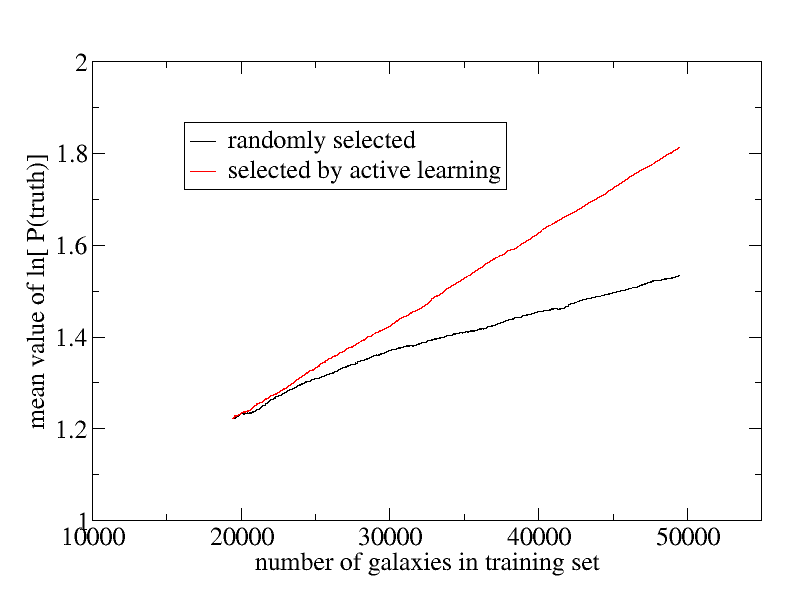
\includegraphics[scale=0.2]{learning_curve.png}
\caption{
A demonstration of the efficacy of Active Learning.
15\% of the 97,000 simulated LSST galaxy observations are randomly
assigned to the training data for our Gaussian Process algorithm.
The black curve shows the performance of the algorithm as more galaxies
are assigned at random to the training data.
The red curve shows the performace of the algorithm as galaxies are chosen
which maximize $-\ln[P(\text{mode})]$ and added to the training data.
Judiciously choosing training galaxies ultimately improves the performance of
our learning algorithm.
}
\label{fig:learning}
\end{figure}

Figure \ref{fig:learning} demonstrates the effect that active learning can
have on an automatic classifier, like our Gaussian Process photometric redshift
algorithm.  Initially, 15\% of our 97,000 simulated LSST galaxy observations are
randomly chosen to be training (spectroscopic) data.  After that, we attempt two
schemes to grow our training set.  The black curve represents random selection
of training data.  The red curve represents training data chosen such that,
at each iteration, the
galaxy with the maximum value of of $F\equiv-\ln[P(\text{mode})]$ is added 
to the
training data.  Choosing to follow up on 
galaxies about
which the least is known (those with maximum $F$) ultimately produces a more
effective classifier.

The method demonstrated above was the simplest possible active learning scheme. 
At each iteration, the algorithm ``greedily'' chose the galaxy with the
least-constraining PDF (measured by the vaule of the PDF at its mode).
More advanced active learning algorithms explored by our group in other contexts
\cite{Garnett11,Garnett12} choose follow-up candidates by ``looking ahead'' and
determining the effect of a follow-up measurement on the expected accuracy of
the classification after both the immediate next iteration and the iteration to
follow.  This algorithm was originally implemented in the case of a binary
classification (``benign'' versus ``malicious'' inputs).  In the current
context, we will extend this analysis to incorporate the full posterior
PDF over redshift.

We will test our algorithms using both real (as in Figure \ref{fig:sdss}) and
simulated (as in Figures \ref{fig:gp} and \ref{fig:learning}) data.
Connolly is
the LSST lead for simulation.  Validation of these techniques will utilize
existing data sets comprising spectroscopic redshifts and five band
photometry for one million galaxies taken from the SDSS (for low redshift
galaxies) and 30,000 galaxies from the
DEEP2\footnote{http://deep.ps.uci.edu} survey (for high redshift galaxies).
We will extend these datasets to include multiple narrow band observations
to evaluate how well we can measure redshifts with narrow band photometry.

\section{Transient Classification}

In addition to the unknown constituents of cosmology, future surveys promise to
yield observations of unknown sources within our own galaxy.  Most exciting
among these will be the variable sources: stars whose luminosity changes either
periodically or cataclysmically.  Some such sources are already known and
well-understood, such as type II supernovae.  
Some are known, but mysterious, such as the afterglows of
Gamma Ray Bursts.
Many others are still waiting to be discovered \cite{sciencebook}.  As with
cosmological redshift, it would be ideal if we could take detailed spectra and
time-series photometry of each source in order to understand its physical
nature.  This is unrealistic.  The LSST is projected to detect as many as one
million variable sources every night \cite{lsstoverview}. 
There are not sufficient follow-up resources to target every one of these
sources with a detailed observation. 
Astronomers must develop algorithms to identify,
in real time, using sparse observations which transients are novel and which are 
well-understood and what follow-up observations would yield the most information
about the novel sources.  These algorithms must be rapid and robust, as the
decision to follow-up a given transient must be made before the transient fades
back into quiescence.  In addition to their impact on future surveys, such as
the LSST, these algorithms will find immediate application characterizing
observations taken by The Palomar Transient
Factory\footnote{http://www.astro.caltech.edu/ptf/} and Catalina Sky
Survey\footnote{http://www.lpl.arizona.edu/css/}.

Real-time automatic classification of objects is already widely acknowledged as a
necessary support technology for the forthcoming age of survey astronomy
\cite{djorgovski2011,richards2011,richards2012,graham2012,mahabal2008a,mahabal2011a}.
Objects will need to be categorized into known science classes so that novel
or rare objects can be flagged for detailed follow-up observations.
For transient events, algorithms must be able to make rapid
decisions so that sources can be targeted for follow-up 
and classifications learned before
objects return to their quiescent phases.  A great deal of work has
already been done developing algorithms that can learn the classification of an
object given a fixed set of observations and training data.  
Mahabal {\it et al}. (2008a,2011a,2011b) propose to break down the
observations of a given object into $\{\Delta m,\Delta t\}$ pairs (where $m$
is magnitude and $t$ is time) and use the density of observations in this 
two-dimensional space as the basis for a Bayesian classification algorithm.
Mahabal {\it et al}. (2008b) alternatively propose to use those same 
$\{\Delta m,\Delta t\}$ pairs as the input to a Gaussian process regression
by which they will reconstruct the object's entire light curve as a function
of time, and then classify the object based on that reconstruction.
Richards {\it et al}. (2011) use observations of transient objects to extract
periodic (e.g. the amplitude and frequency of the first two Fourier modes of
the object's light curve) and non-periodic (e.g. the variance and skewness of
all of the magnitude observations taken, regardless of their separation in
time) and feed those features into several tree-based classifiers.
They find misclassification rates lower than 30\% with their best method yielding a
misclassification rate of 22.8\%.  Using only non-periodic features, which will be
especially easy for survey telescopes to gather, rather than
full light curves, they 
find a misclassification rate of
between 26\% and 28\%.
Bloom {\it et al}. (2011) also use a tree-based automatic classifier on
Palomar Transient Factory data and find a 3.8\% error rate when
discriminating between four major classifications.  Richards {\it et al}.
consider a more complete set of 25 possible classifications.
Clearly, many possibile approaches are available for the automated
classification of transient objects, and not all of them rely upon highly
detailed observations to function.

\subsection{Active Learning for Transient Objects}

The input features for transient object classification will be photometric
and morphologic measures taken at different increments in time.  The output
is a categorical variable indicating the class.  This is in contrast to
photometric redshifts where the output is continuous.  Fortunately, the
underlying covariance for Gaussian process classification is the same as
for regression and we will adopt a similar prediction model.

The active learning problem for transient objects contains three
subproblems, active learning, active search, and active feature
acquisition.  Finally, one additional difference between the transient
object method and the photometric redshift method is that transient object
decisions must be made in an online, streaming fashion.  Rather than
considering an entire pool of test objects, they appear one at a time as
they are detected and the algorithm must decide whether and how to follow
up on each immediately as they are detected.  We first describe algorithms
for each of the three pieces and then how to combine them into a single
algorithm for streaming transient detections.

{\bf Active Learning.} In order to get a ground-truth class for a transient
object, repeated observations are taken to estimate a full light curve.  A
human expert then assigns a class label.  Both the repeated telescope
observations and human time are expensive and thus we want to learn a good
classification model using limited training data.  We propose a
corresponding trace and survey criteria for active learning on transients
as in Section \ref{sec:mlpz}.

{\bf Active Feature Acquisition.} When considering photometric redshifts,
we assumed that all photometric inputs were observed for every object of
interest.  For transients this will not be the case.  A large component of
the problem is deciding for each object, whether observations of additional
colors and/or additional times would be valuable in classifying or
characterizing the object.

We propose to extend our recent work on using GPs to detect damped
lyman-alpha (DLA) systems \cite{Garnett12a}.  In that work GP regression
was used on each observed, noisy spectrum to infer the latent spectrum.
The single independent (input) variable was wavelength.  For transient
objects we will have 5 color magnitudes that are a function of time and are
coupled to each other.  In the DLA work, a different model was learned for
spectra with and without a DLA.  DLAs were classified by recognizing which
model fit best.  In the proposed work, we will learn a different model for
each class of object and will estimate class probabilities using Bayes rule
for combining the prior probability for each class and how well the
respective models fit the observations.  The key advantage of this approach
is that the GPs naturally provide a mean and covariance for future
unobserved colors.  This uncertainty propagates through to class labels and
we can use it to estimate the reduction in class uncertainty that will be
gained by observing a certain color at a certain time.  The observation
yielding the greatest reduction in entropy for the class and the light
curves for this object will be taken.

{\bf Active Search.} Many transient objects will be from common and/or 
well-understood classes that do not have much observational value.  The ultimate
objective in following up detected transients is to maximize the number of
interesting transients classified and characterized while staying within a
budget of follow-up observations.  This is an active search problem. The
problem and the Bayesian optimal algorithm for it are described in our
recent work \cite{Garnett11,Garnett12}.  As in active learning, the
acquisition of class labels is expensive and we need to learn a model to
predict these labels from limited input data.  However, the final
performance objective is not the accuracy of the classifier, but rather the
number of positives (i.e. objects from interesting classes) identified.  We
propose to use the simple myopic algorithm described in that work.  It
computes the probability of each point belonging to the positive class and
chooses the largest.


{\bf A combined streaming method.} The three goals above will be combined
in a staged set of decisions.  When a new transient is detected, the light
curve model will be used to provide estimated light curves for the object.
Those light curves are the input variables for this object in the active
learning and active search algorithms.  In parallel, the active learning
and active search methods will decide whether to follow up on this object.
If either of them selects the object, it is advanced to active feature
acquisition.  There additional observations on the object are selected and
the process for this object repeats.  An object that initially seemed
interesting to one algorithm may cease to be so after additional
observations or may be adopted by the other one.  The process for one
object terminates when neither active learning nor active search remains
interested in it or the object class and light curves are characterized
well enough that no more observations are required.

The active search and active learning algorithms each compute an objective
criterion score for each object.  For photometric redshifts the scores are
used to create a ranked list and observations are scheduled proceeding down
the list.  When a budget is given for follow-ups on each batch of newly
detected transients, going down a ranked list in each batch until that
budget is exhausted is appropriate.

However, when the budget is an aggregate over a longer time period a
streaming decision on how much of the budget to spend on each batch must be
made on that batch in isolation.  This will be done by choosing a score
threshold.  The threshold will be set by evaluating the historical stream
and setting it at a value that would yield a number of follow ups equal to
an available budget for following up.  The threshold will be adjusted
continuously as more observations are taken and the models and scientific
goals change (e.g. the object types designated as ``interesting'' are
changed).

Since all of the algorithm components are based on GP models, it is
possible to merge them together into a single model.  We hypothesize that
additional performance improvements can be made through an integrated model
and decision algorithm.  For example, an object with a modest active
learning score that can be easily characterized with only one more follow
up might be promoted over one with a higher score that can not be easily
characterized even with many more observations.  After we have implemented
the staged method described above, we will investigate and compare an
integrated model.


\section{On-Line Learning Algorithms}

\newpage
%%%%%%%%%%%%%%%%%%%%%%%%%%%%%%%%%%%%%%%%%%%%%%%%%%%%%%%%%%%%
%%%%%%%%%%%%%%%%%%%%%%%%%%%%%%%%%%%%%%%%%%%%%%%%%%%%%%%%%%%%

%%%%%%%%%%%%%%%%%%%%%%%%%%%%%%%%%%%%%%%%%%%%%%%%%%%%%%%%%%%%
%%%%%%%%%%%%%%%%%%%%%%%%%%%%%%%%%%%%%%%%%%%%%%%%%%%%%%%%%%%%
\begin{thebibliography}{99}

\bibitem[Abazajian {\it et al}. 2009]{Abazajian:2008wr}
  Abazajian, K.~N.{\it et al.}  [SDSS Collaboration]~2009,
  %``The Seventh Data Release of the Sloan Digital Sky Survey,''
  The Astrophysical Journal Supplement Series  {\bf 182}, 543
  [arXiv:0812.0649 [astro-ph]].
  %%CITATION = APJSA,182,543;%%

\bibitem[Abdalla {\it et al}. 2011]{abdalla}
Abdalla,~F.~B., Banerji,~M., Lahav,~O., and Rashkov,~V. 2011,
Monthly Notices of the Royal Astronomical Society {\bf 417}, 1891

\bibitem[Abramo {\it et al}. 2012]{narrow}
Abramo,~L.~R., Strauss,~M.~A., Lima,~M., Hern\'andez-Monteagudo,~C., Lazkoz,~R.,
Moles,~M., de Oliveira,~C.~M., Sendra,~I., Sodr\'e Jr.,~L., and
Storchi-Bergmann,~T. 2012, Monthly Notices of the Royal Astronomical Society
{\bf 423}, 3251

\bibitem[Albrecht {\it et al}. 2006]{detf}
Albrecht,~A., Bernstein,~B., Cahn,~R., Freedman,~W.~L., Hewitt,~J.,
Hu,~W., Huth,~J., Kamionkowski,~M., Kolb,~E., Knox,~L., Mather,~J.~C.,
Staggs,~S., Suntzeff,~N.~B. (Dark Energy Task Force) 2006,
``Report of the Dark Energy Task Force,''
\verb|http://jdem.gsfc.nasa.gov/science/DETF_Report.pdf|


\bibitem[Berg\'e {\it et al}. 2012]{psf}
Berg\'e,~J., Price,~S., Amara,~A., and Rhodes,~J. 2012,
Monthly Notices of the Royal Astronomical Society {\bf 419}, 2356

\bibitem[Bloom {\it et al}. 2011]{bloom2011}
Bloom,~J.~S., Richards,~J.~W., Nugent,~P.~E., Quimby,~R.~M., Kasliwal,~M.~M.,
Starr,~D.~L., Posnanski,~D., Ofek,~E.~O., Cenko,~S.~B., Butler,~N.~R.,
Kulkarni,~S.~R., Gal-Yam,~A., and Law,~N. 2011 [arXiv:1106.5491]

\bibitem[Bonfield {\it et al}. 2010]{Bonfield}
Bonfield,~D.~G., Sun,~Y., Davey,~N., Jarvis,~M.~J., Abdalla,~F.~B.,
Banerji,~M., Adams,~R.~G. 2010, Monthly Notices of the Royal Astronomical Society 
{\bf 405} 987

\bibitem[Brammer {\it et al}. 2008]{eazy}
Brammer,~G.~B., van Dokkum,~P.~G., and Coppi,~P. 2008,
The Astrophysical Journal {\bf 686}, 1503

\bibitem[Bryan 2007]{brentsthesis}
Bryan, B., 2007, Ph.D. thesis
\verb|http://reports-archive.adm.cs.cmu.edu/anon/|
\verb|ml2007/abstracts/07-122.html|

\bibitem[Bryan {\it et al}. 2007]{bryan}
Bryan, B., Schneider, J., Miller, C.~J., Nichol, R.~C., Genovese, C., and
Wasserman, L., 2007,
The Astrophysical Journal {\bf 665}, 25

\bibitem[Budav\'ari 2008]{budavari2008}
Budav\'ari,~T. 2008 The Astrophysical Journal {\bf 695}, 747

\bibitem[Collister and Lahav 2004]{annz}
Collister,~A.~A. and Lahav,~O. 2004,
Publications of the Astronomical Society of the Pacific {\bf 116}, 345

\bibitem[Connolly {\it et al}. 2005]{imsim}
Connolly,~A.~J., Peterson,~J., Jernigan,~J.~G., Abel,~R., Bankert,~J.,
Chang,~C., Claver,~C.~F., Gibson,~R., Gilmore,~D.~K., Grace,~E., Jones,~R.~L.,
Ivezic,~Z., Jee,~J., Juric,~M., Kahn,~S.~M., Krabbendam,~V.~L., Krughoff,~S.,
Lorenz,~S., Pizagno,~J., Rasmussen,~A., Todd,~N. Tyson,~J.~A., and Young,~M.
2005, Society of the Photo-Optical Instrumentation Engineers (SPIE) Converence
Series {\bf 7738}, 53

\bibitem[Cunha {\it et al}. 2012]{cunha2012}
Cunha,~C.~E., Huterer,~D., Lin,~H., Busha,~M.~T., and Wechsler,~R.~H. 2012,
[arXiv:1207.3347]

\bibitem[Daniel and Linder 2010]{muvarpi2}
Daniel,~S.~F. and Linder,~E.~V. 2010, Physical Review D {\bf 82}, 103523

%\cite{Daniel:2011rr}
\bibitem[Daniel {\it et al}. 2011]{daniel2011} 
  Daniel,~S.~F., Connolly,~A.~J., Schneider,~J., Vanderplas,~J. and Xiong,~L. 
  %``Classification of Stellar Spectra with LLE,''
  The Astronomical Journal  {\bf 142}, 203 (2011)
  [arXiv:1110.4646 [astro-ph.SR]].
  %%CITATION = ARXIV:1110.4646;%%

\bibitem[Daniel {\it et al}. 2012]{daniel2012}
Daniel,~S.~F., Connolly,~A.~J., and Schneider,~J. 2012
[arXiv:1205.2708]

\bibitem[Das {\it et al}. 2011]{sudeep}
Das,~S., de Putter,~R., Linder,~E.~V., and Nakajima,~R. 2011,
[arXiv:1102.5090]

\bibitem[Davis {\it et al}. 2007]{essence}
Davis,~T.~M., M\"ortsell,~E., Sollerman,~J., Becker,~A.~C., Blondin,~S.,
Challis,~P., Clocchiatti,~A., Filippenko,~A.~V., Foley,~R.~J., Garnavich,~P.~M.,
Jha,~S., Krisciunas,~K., Kirshner,~R.~P., Leibundgut,~B., Li,~W., Matheson,~T.,
Miknaitis,~G., Pignata,~G., Rest,~A., Riess,~A.~G., Schmidt,~B.~P.,
Smith,~R.~C., Spyromilio,~J., Stubbs,~C.~W., Suntzeff,~N.~B., Tonry,~J.~L.,
Wood-Vasey,~W.~M., and Zenteno,~A. 2007, The Astrophysical Journal, {\bf 666},
716

\bibitem[de Putter {\it et al}. 2010]{roland}
de Putter,~R., Huterer,~D. and Linder,~E.~V. 2010, Physical Review D {\bf 81},
103513


\bibitem[Djorgovski {\it et al}. 2011]{djorgovski2011}
Djorgovski,~S.~J., Donalek,~C., Mahabal,~A.~A., Moghaddam,~B., Turmon,~M.,
Graham,~M.~J., Drake,~A.~J., Sharma,~N. and Chen,~Y. 2011
[arXiv:1110.4655] to appear in Statistical Analysis and Data Mining, ref. proc.
CIDU 2011 conf., eds. A. Srivastava and N. Chawla

\bibitem[Garnett {\it et al}. 2011]{Garnett11}
Garnett,~R., Krishnamurhty,~Y., Wang,~D., Schneider,~J., and Mann,~R. 2011,
``Bayesian Optimal Active Search on Graphs,'' KDD Workshop on Mining and
Learning with Graphs

\bibitem[Garnett {\it et al}. 2012a]{Garnett12}
Garnett,~R., Krishnamurthy,~Y., Xiong,~X., Schneider,~J., and Mann,~R. 2012a,
``Bayesian Optimal Active Search and Surveying,'' International Conference on
Machine Learning

\bibitem[Garnett {\it et al}. 2012b]{Garnett12a}
Garnett,~R., Ho,~S., and Schneider,~J. 2012b,
``Gaussian Processes for Identifying Damped Lyman-alpha Systems in Spectroscopic
Surveys,'' Neural Information Processing Systems 
workshop on Modern Nonparametric Methods in Machine Learning

\bibitem[Graham {\it et al}. 2012]{graham2012}
Graham,~M.~J., Djorgovski,~S.~G., Mahabal,~A., Donalek,~C., Drake,~A.,
Longo,~G. 2012 [arXiv:1208.2480] to appear in special issue of Distributed and
Parallel Databases on Data Intensive eScience

\bibitem[Huterer {\it et al}. 2006]{huterer2006}
Huterer,~D., Takada,~M., Bernstein,~G., and Jain,~B. 2006,
Monthly Notices of the Royal Astronomical Society {\bf 366}, 101

\bibitem[Kitching {\it et al}. 2008]{kitching}
Kitching,~T.~D., Taylor,~A.~N., and Heavens,~A.~F. 2008,
Monthly Notices of the Royal Astronomical Society {\bf 389} 173

\bibitem[Long {\it et al}. 2012]{long2012}
Long,~J.~P., El Karoui,~N., Rice,~J.~A., Richards,~J.~W., and Bloom,~J.~S. 2012,
Publications of the Astronomical Society of the Pacific {\bf 124} 280

\bibitem[LSST Collaboration 2011]{lsstoverview}
LSST Collaboration 2011, [arXiv:0805.2366]
\verb|http://www.lsst.org/lsst/overview/|

\bibitem[LSST Dark Energy Science Collaboration 2012]{desc}
LSST Dark Energy Science Collaboration 2012, [arXiv:1211.0310]

\bibitem[LSST Science Collaborations 2009]{sciencebook}
LSST Science Collaborations 2009, ``LSST Science Book'',
\verb|http://www.lsst.org/lsst/science/scibook|

\bibitem[Ma {\it et al}. 2006]{Ma2006}
Ma,~Z., Hu,~H., and Huterer,~D. 2006, The Astrophysical Journal {\bf 636}, 21

\bibitem[Ma {\it et al}. 2012]{YifeiMa12}
Ma,~Y., Garnett,~R., and Schneider,~J. 2012,
``Submodularity in Batch Active Learning and Survey Problems
on Gaussian Random Fields,''
Neural Information Processing Systems 
workshop on Discrete Optimization in Machine Learning

\bibitem[Mahabal {\it et al}. 2008a]{mahabal2008a}
Mahabal,~A., Djorgovski,~S.~G., Turmon,~M., Jewell,~J., Williams,~R.~R.,
Drake,~A.~J., Graham,~M.~G., Donalek,~C., Glikman,~E., and the Palomar-QUEST Team
2008a, Astronomische Nachrichten {\bf 329}, 288

\bibitem[Mahabal {\it et al}. 2008b]{mahabal2008b}
Mahabal,~A., Djorgovski,~S.~G., Williams,~R., Drake,~A., Donalek,~C.,
Graham,~M., Moghaddam,~B., Turmon,~M., Jewell,~J., Khosla,~A., and
Hensley,~B. 2008b [arXiv:0810.4527] to appear in proceedings fo the Class2008
conference (Classification and Discovery in Large Astronomical Surveys, Ringberg
Castle, 14-17 October 2008)

\bibitem[Mahabal {\it et al}. 2011a]{mahabal2011a}
Mahabal,~A.~A., Donalek,~C., Djorgovski,~S.~J., Drake,~A.~J.,
Graham,~M.~J., Williams,~R., Chen,~Y., Moghaddam,~B., and Turmon,~M.
2011a, [arxiv:1111.3699] to appear in Proc. IAU 285, ``New Horizons in Transient
Astronomy,'' Oxford, September 2011

\bibitem[Mahabal {\it et al}. 2011b]{mahabal2011b}
Mahabal,~A.~A., Djorgovski,~S.~G., Drake,~A.~J., Donalek~C., Graham,~M~J.,
Williams,~R.~D., Chen,~Y., Moghaddam,~B., Turmon,~M., Beshore,~E., and Larson,~S.
2011b, Bulletin of the Astronomical Society of India {\bf 39}, 387

\bibitem[Mandelbaum {\it et al}. 2008]{mandelbaum2008}
Mandelbaum,~R., Seljak,~U., Hirata,~C.~M., Bardelli,~S., Bolzonella,!M.,
Bongiorno,~A., Carollo,~M., Contini,~T., Cunha,~C.~E., Garilli,~B.,
Iovino,~A., Kambczyk,~P, Kneib,~J.-P., Knobel,~C., Koo,~D.~C., Lamareille,~F.,
Le F\`evre,~O., Leborgne,~J.-F., Lilly,~S.~J., Maier,~C., Mainieri,~V.,
Mignoli,~M., Newman,~J.~A., Oesch,~P.~A., Perez-Montero,~E., Ricciardelli,~E.,
Scodeggio,~M., Silverman,~J., and Tasca,~L. 2008, Monthly Notices of the Royal
Astronomical Society {\bf 386}, 781

\bibitem[McBride {\it et al}. 2011a]{mcbride2011a}
McBride,~C.~K., Connolly,~A.~J., Gardner,~J.~P., Scranton,~R., Newman,~J.~A.,
Scoccimarro,~R., Zehavi,~I., and Schneider,~D.~P. 2011a, The Astrophysical
Journal, {\bf 726}, 13

\bibitem[McBride {\it et al}. 2011b]{mcbride2011b}
McBride,~C.~K., Connolly,~A.~J., Gardner,~J.~P., Scranton,~R., Scoccimarro,~R.,
Berlind,~A.~A., Mar\'in,~F., and Schneider,~D.~P. 2011b, The Astrophysical
Journal {\bf 739}, 85

\bibitem[Moore {\it et al}. 2000]{Moore00}
Moore,~A., Connolly,~A., Genovese,~C., Grone,~L., Kanidoris,~N., Nichol,~R.,
Schneider,~J., Szalay,~A., Szapudi,~I., and Wasserman,~L. 2000,
``Fast Algorithms and Efficient Statistics: N-point Correlation Functions,'' in
MPA/MPE/ESO Conference on Mining the Sky [arXiv:astro-ph/0012333]

\bibitem[Nakajima {\it et al}. 2012]{nakajima2011}
Nakajima,~R., Mandelbaum,~R., Seljak,~U., Cohn,~J.~D., Reyes,~R., and
Cool,~R. 2012, Monthly Notices of the Royal Astronomical Society {\bf 420}, 3240
[arXiv:1107.1395]

\bibitem[Nichol {\it et al}. 2006]{Nichol2006}
Nichol,~R.~C., Sheth,~R.~K., Suto,~Y., Gray,~A.~J., Kayo,~I., Wechsler,~R.~H.,
Marin,~F., Kulkarni,~G., Blanton,~M., Connolly,~A.~J., Gardner,~J.~P., Jain,~B.,
Miller,~C.~J., Moore,~A.~W., Pope,~A., Pun,~J., Schneider,~D., Schneider,~J.,
Szalay,~A., Szapudi,~I., Zehavi,~I., Bahcall,~N.~A., Csabai,~I., Brinkmann,~J.
2006, Monthly Notices of the Royal Astronomical Society {\bf 368}, 1507

\bibitem[Poczos and Schneider 2011]{poczos11alphadiv}
Poczos,~B. and Schneider,~J. 2011, ``On the Estimation of alpha-Divergences,''
Artificial Intelligence and Statistics (AISTATS)

\bibitem[Poczos {\it et al}. 2011]{Poczos2011UAI}
Poczos,~B., Xiong,~L., and Schneider,~J. 2011, ``Nonparametric Divergence Estimation with
Applications to Machine Learning on Distributions,''  Uncertainty in Artificial
Intelligence

\bibitem[Poczos {\it et al}. 2012]{poczos12CVPR}
Poczos,~B., Xiong,~L., Sutherland,~D., and Schneider,~J. 2012,
``Nonparametric Kernel Estimators for Image Classification,''
IEEE Conference on Computer Vision and Pattern Recognition

\bibitem[Rasmussen and Williams 2006]{gp}
Rasmussen, C.~E. and Williams, C.~K.~I., 2006, ``Gaussian
Processes for Machine Learning''
\verb|http://www.GaussianProcess.org/gpml/|

\bibitem[Richards {\it et al}. 2004]{qso}
Richards,~G.~T., Nichols,~R.~C., Gray,~A.~G., Brunner,~R.~J., Lupton,~R.~H.,
Vanden Berk,~D.~E., Chong,~S.~S., Weinstein,~M.~A., Schneider,~D.~P.,
Anderson,~S.~F., Munn,~J.~A., Harris,~H.~C., Strauss,~M.~A., Fan,~X.,
Gunn,~J.~E., Ivezi\'c,~Z., York,~D.~G., Brinkmann,~J., and Moore,~A.~W. 2004,
The Astrophysical Journal Supplement Series, {\bf 155}, 257

\bibitem[Richards {\it et al}. 2011]{richards2011}
Richards,~J.~W., Starr,~D.~L., Butler,~N.~R., Bloom,~J.~S., Brewer,~J.~M.,
Crellin-Quick,~A., Higgins,~J., Kennedy,~R., and Rischard,~M. 2011,
The Astrophysical Journal {\bf 733}, 10

\bibitem[Richards {\it et al}. 2012]{richards2012}
Richards,~J.~W., Starr,~D.~L., Brink,~H., Miller,~A.~A., Bloom,~J.~S.,
Butler,~N.~R., James,~J.~B., Long,~J.~P., and Rice,~J. 2012
The Astrophysical Journal {\bf 744}, 192

\bibitem[Rosenfield {\it et al}. 2011]{rosenfield2011}
Rosenfield,~P., Connolly,~A., Fay,~J., Sayres,~C., and Tofflemire,~B. 2011,
Astronomical Society of the Pacific Conference Series {\bf 443}, 109

\bibitem[Scranton {\it et al}. 2002]{Scranton2002}
Scranton,~R., Johnston,~D., Dodelson,~S., Frieman,~J.~A., Connolly,~A.,
Eisenstein,~D.~J., Gunn,~J.~E., Hui,~L., Jain,~B., Kent,~S., Loveday,~J.,
Narayanan,~V., Nichol,~R.~C., O'Connell,~L., Soccimarro,~R., Sheth,~R.~K.,
Stebbins,~A., Strauss,~M.~A., Szalay,~A.~S., Sapudi,~I., Tegmark,~M.,
Vogeley,~M., Zehavi,~I., Annis,~J., Bahcall,~N.~A., Brinkman,~J., Csabai,~I.,
Hindsley,~R., Ivezic,~Z., Kim,~R.~S.~J., Knapp,~G.~R., Lamb,~D.~Q., Lee,~B.~C.,
Lupton,~R.~H., McKay,~T., Munn,~J., Peoples,~J., Pier,~J., Richards,~G.~T.,
Rockosi,~C., Schlegel,~D., Schneider,~D.~P., Stoughton,~C., Tucker,~D.~L.,
Yanny,~B., York,~D.~G. 2002, The Astrophysical Journal {\bf 579}, 48

\bibitem[Sesar {\it et al}. 2011]{linear}
Sesar,~B., Stuart,~J.~S., Ivezi\'c,~\u Z., Morgan,~D.~P., Becker,~A.~C., and
Wo\'zniak,~P. 2011, The Astronomical Journal {\bf 142}, 190

\bibitem[Settles 2009]{activelearning}
Settles,~B. 2009, ``Active Learning Literature Survey,'' Computer Sciences Technical
Report 1648, University of Wisconsin-Madison,
\verb|http://pages.cs.wisc.edu/~bsettles/active-learning/|


\bibitem[Shafieloo {\it et al}. 2012]{ericgp}
Shafieloo,~A., Kim,~A.~G., and Linder,~E.~V. 2012,
Physical Review D {\bf 85}, 123530 [arXiv:1204.2272]


\bibitem[Skibba {\it et al}. 2006]{Skibba2006}
Skibba,~R., Sheth,~R.~K., Connolly,~A.~J., and Scranton,~R. 2006,
Monthly Notices of the Royal Astronomical Society, {\bf 369}, 68

\bibitem[Straf 2003]{straf03}
Straf,~M.~L. 2003, Journal of the American Statistical Association {\bf 98}, 1

\bibitem[Szapudi {\it et al}. 2002]{Szapudi2002}
Szapud,~I., Frieman,~J.~A., Scoccimarro,~R., Szalay,~A.~S., Connolly,~A.~J.,
Dodelson,~S., Eisenstein,~D.~J., Gunn,~J.~E., Johnston,~D., Kent,~S.,
Loveday,~J., Meiksin,~A., Nichol,~R.~C., Scranton,~R., Stebbins,~A.,
Vogeley,~M.~S., Annis,~J., Bahcall,~N.~A., Brinkman,~J., Csabai,~I., Doi,~M.,
Fukigita,~M., Ivezi\'c,~\u Z., Kim,~R.~S.~J., Knapp,~G.~R., Lamb,~D.~Q.,
Lee,~B.~C., Lupton,~R.~H., McKay,~T.~A., Munn,~J., Peoples,~J., Pier,~J.,
Rockosi,~C., Schlegel,~D., Stoughtfon,~C., Tucker,~D.~L., Yanny,~B., York,~D.~G.
2002, The Astrophysical Journal {\bf 570}, 75

\bibitem[Vanderplas and Connolly 2009]{vdp2009}
Vanderplas,~J. and Connolly,~A.~J. 2009,
Astronomical Journal {\bf 138}, 1365

\bibitem[Wiley {\it et al}. 2011]{wiley2011}
Wiley,~K, Connolly,~A.~J., Gardner,~J., Krughoff,~S., Balazinska,~M., Howe,~B.,
Kwon,~Y., and Bu, ~Y. 2011, Publication of the Astronomical Society of the
Pacific {\bf 123}, 366

\bibitem[Xiong {\it et al}. 2011a]{Xiong2011gad}
Xiong,~L., Poczos,~B., Schneider,~J., Connolly,~A., Vanderplas,~J. 2011a,
``Hierarchical Probabilistic Models for Group Anomaly Detection,''
Artificial Intelligence and Statistics (AISTATS)

\bibitem[Xiong {\it et al}. 2011b]{xiong2011fgm}
Xiong,~L., Poczos,~B., and Schneider,~J. 2011, ``Group Anomaly Detection using Flexible
Genre Models,'' Neural Information Processing Systems

\bibitem[Yip {\it et al}. 2004]{yip2004a}
Yip,~C.~W., Connolly,~A.~J., Szalay,~A.~S., Budav\'ari,~T., SubbaRao,~M.,
Frieman,~J.~A., Nichol,~R.~C., Hopkins,~A.~M., York,~D.~G., Okamura,~S.,
Brinkmann,~J., Csabai,~I., Thakar,~A.~R., Fukugita,~M., 
and Ivezi\'c,~\u Z. 2004, The Astronomical Journal {\bf 128}, 585

\bibitem[Zhang and Schneider 2010a]{YiZhangICML2010}
Zhang,~Y. and Schneider,~J. 2010a, ``Projection Penalties: Dimension Reduction without
Loss,'' International Conference on Machine Learning

\bibitem[Zhang and Schneider 2010b]{YiZhangMultitask2010}
Zhang,~Y. and Schneider,~J. 2010b,
``Learning Multiple Tasks with a Sparse Matrix-Normal Penalty,''
Neural Information Processing Systems

\bibitem[Zhang {\it et al}. 2010]{YiZhangSDM2010}
Zhang,~Y., Schneider,~J., and Dubrawski,~A. 2010,
``Learning Compressible Models,'' Proceedings of SIAM Data Mining Conference

\bibitem[Zhang and Schneider 2011]{YiZhang2011multiECOC}
Zhang,~Y. and Schneider,~J 2011, ``Multi-label Output Codes using Canonical Correlation
Analysis,'' Artificial Intelligence and Statistics

\bibitem[Zhang and Schneider 2012]{YiZhang2012}
Zhang,~Y. and Schneider,~J. 2012, ``Maximum Margin Output Coding,''
International Conference on Machine Learning

\end{thebibliography} 
\label{lastpage}

\end{document}

%%%%%%%%%%%%%%%%%%%%%%%%%%%%%%%%%%%%%%%%%%%%%%%%%%%%%%%%%%%%
